% Options for packages loaded elsewhere
\PassOptionsToPackage{unicode}{hyperref}
\PassOptionsToPackage{hyphens}{url}
%
\documentclass[
]{article}
\usepackage{amsmath,amssymb}
\usepackage{lmodern}
\usepackage{iftex}
\ifPDFTeX
  \usepackage[T1]{fontenc}
  \usepackage[utf8]{inputenc}
  \usepackage{textcomp} % provide euro and other symbols
\else % if luatex or xetex
  \usepackage{unicode-math}
  \defaultfontfeatures{Scale=MatchLowercase}
  \defaultfontfeatures[\rmfamily]{Ligatures=TeX,Scale=1}
\fi
% Use upquote if available, for straight quotes in verbatim environments
\IfFileExists{upquote.sty}{\usepackage{upquote}}{}
\IfFileExists{microtype.sty}{% use microtype if available
  \usepackage[]{microtype}
  \UseMicrotypeSet[protrusion]{basicmath} % disable protrusion for tt fonts
}{}
\makeatletter
\@ifundefined{KOMAClassName}{% if non-KOMA class
  \IfFileExists{parskip.sty}{%
    \usepackage{parskip}
  }{% else
    \setlength{\parindent}{0pt}
    \setlength{\parskip}{6pt plus 2pt minus 1pt}}
}{% if KOMA class
  \KOMAoptions{parskip=half}}
\makeatother
\usepackage{xcolor}
\IfFileExists{xurl.sty}{\usepackage{xurl}}{} % add URL line breaks if available
\IfFileExists{bookmark.sty}{\usepackage{bookmark}}{\usepackage{hyperref}}
\hypersetup{
  pdftitle={Estatística básica},
  hidelinks,
  pdfcreator={LaTeX via pandoc}}
\urlstyle{same} % disable monospaced font for URLs
\usepackage[margin=1in]{geometry}
\usepackage{color}
\usepackage{fancyvrb}
\newcommand{\VerbBar}{|}
\newcommand{\VERB}{\Verb[commandchars=\\\{\}]}
\DefineVerbatimEnvironment{Highlighting}{Verbatim}{commandchars=\\\{\}}
% Add ',fontsize=\small' for more characters per line
\usepackage{framed}
\definecolor{shadecolor}{RGB}{248,248,248}
\newenvironment{Shaded}{\begin{snugshade}}{\end{snugshade}}
\newcommand{\AlertTok}[1]{\textcolor[rgb]{0.94,0.16,0.16}{#1}}
\newcommand{\AnnotationTok}[1]{\textcolor[rgb]{0.56,0.35,0.01}{\textbf{\textit{#1}}}}
\newcommand{\AttributeTok}[1]{\textcolor[rgb]{0.77,0.63,0.00}{#1}}
\newcommand{\BaseNTok}[1]{\textcolor[rgb]{0.00,0.00,0.81}{#1}}
\newcommand{\BuiltInTok}[1]{#1}
\newcommand{\CharTok}[1]{\textcolor[rgb]{0.31,0.60,0.02}{#1}}
\newcommand{\CommentTok}[1]{\textcolor[rgb]{0.56,0.35,0.01}{\textit{#1}}}
\newcommand{\CommentVarTok}[1]{\textcolor[rgb]{0.56,0.35,0.01}{\textbf{\textit{#1}}}}
\newcommand{\ConstantTok}[1]{\textcolor[rgb]{0.00,0.00,0.00}{#1}}
\newcommand{\ControlFlowTok}[1]{\textcolor[rgb]{0.13,0.29,0.53}{\textbf{#1}}}
\newcommand{\DataTypeTok}[1]{\textcolor[rgb]{0.13,0.29,0.53}{#1}}
\newcommand{\DecValTok}[1]{\textcolor[rgb]{0.00,0.00,0.81}{#1}}
\newcommand{\DocumentationTok}[1]{\textcolor[rgb]{0.56,0.35,0.01}{\textbf{\textit{#1}}}}
\newcommand{\ErrorTok}[1]{\textcolor[rgb]{0.64,0.00,0.00}{\textbf{#1}}}
\newcommand{\ExtensionTok}[1]{#1}
\newcommand{\FloatTok}[1]{\textcolor[rgb]{0.00,0.00,0.81}{#1}}
\newcommand{\FunctionTok}[1]{\textcolor[rgb]{0.00,0.00,0.00}{#1}}
\newcommand{\ImportTok}[1]{#1}
\newcommand{\InformationTok}[1]{\textcolor[rgb]{0.56,0.35,0.01}{\textbf{\textit{#1}}}}
\newcommand{\KeywordTok}[1]{\textcolor[rgb]{0.13,0.29,0.53}{\textbf{#1}}}
\newcommand{\NormalTok}[1]{#1}
\newcommand{\OperatorTok}[1]{\textcolor[rgb]{0.81,0.36,0.00}{\textbf{#1}}}
\newcommand{\OtherTok}[1]{\textcolor[rgb]{0.56,0.35,0.01}{#1}}
\newcommand{\PreprocessorTok}[1]{\textcolor[rgb]{0.56,0.35,0.01}{\textit{#1}}}
\newcommand{\RegionMarkerTok}[1]{#1}
\newcommand{\SpecialCharTok}[1]{\textcolor[rgb]{0.00,0.00,0.00}{#1}}
\newcommand{\SpecialStringTok}[1]{\textcolor[rgb]{0.31,0.60,0.02}{#1}}
\newcommand{\StringTok}[1]{\textcolor[rgb]{0.31,0.60,0.02}{#1}}
\newcommand{\VariableTok}[1]{\textcolor[rgb]{0.00,0.00,0.00}{#1}}
\newcommand{\VerbatimStringTok}[1]{\textcolor[rgb]{0.31,0.60,0.02}{#1}}
\newcommand{\WarningTok}[1]{\textcolor[rgb]{0.56,0.35,0.01}{\textbf{\textit{#1}}}}
\usepackage{graphicx}
\makeatletter
\def\maxwidth{\ifdim\Gin@nat@width>\linewidth\linewidth\else\Gin@nat@width\fi}
\def\maxheight{\ifdim\Gin@nat@height>\textheight\textheight\else\Gin@nat@height\fi}
\makeatother
% Scale images if necessary, so that they will not overflow the page
% margins by default, and it is still possible to overwrite the defaults
% using explicit options in \includegraphics[width, height, ...]{}
\setkeys{Gin}{width=\maxwidth,height=\maxheight,keepaspectratio}
% Set default figure placement to htbp
\makeatletter
\def\fps@figure{htbp}
\makeatother
\setlength{\emergencystretch}{3em} % prevent overfull lines
\providecommand{\tightlist}{%
  \setlength{\itemsep}{0pt}\setlength{\parskip}{0pt}}
\setcounter{secnumdepth}{-\maxdimen} % remove section numbering
\ifLuaTeX
  \usepackage{selnolig}  % disable illegal ligatures
\fi

\title{Estatística básica}
\author{}
\date{\vspace{-2.5em}}

\begin{document}
\maketitle

{
\setcounter{tocdepth}{1}
\tableofcontents
}
{[}EM CONSTRUÇÃO{]}

~

~

\hypertarget{anuxe1lise-de-regressuxe3o}{%
\section{Análise de Regressão}\label{anuxe1lise-de-regressuxe3o}}

~

Os métodos de análise de regressão formam um conjunto de poderosas
ferramentas estatisticas, que estudam a relação entre duas ou mais
variaveis. Por ser de facil interpretação, essas ferramentas podem se
aplicar nas mais diversas àreas e situações, como por exemplo: faixa
salarial e nível de educação, consumo de açúcar e percentual de gordura,
quantidade de fertilizante e crescimento da planta, quantidade gasta em
publicidade e quantidade de vendas de um produto, consumo de contéudo na
TV e faixa etária, etc. Esse conjunto de ferramentas nos permite lidar
com os três tópicos mais comuns quando se trata de regressão:

\begin{itemize}
\tightlist
\item
  \textbf{Modelagem:} Cria uma equação que descreve a relação entre as
  variáveis em questão,de forma parcimoniosa;
\item
  \textbf{Covariância:} Estuda a variação entre as variâveis que
  aparentemente não tem relação entre si;
\item
  \textbf{Predição:} Estima os resultados do modelo para situações
  incertas.
\end{itemize}

O termo regressão foi criado por Francis Galton no século 19 durante seu
estudo sobre a relação entre a altura de pais e filhos, desenvolvido no
artigo
\href{https://galton.org/essays/1880-1889/galton-1886-jaigi-regression-stature.pdf}{\emph{Regression
Toward Mediocrity in Hereditary Stature}}. Hoje aplicamos estas tecnicas
com o apoio da programação, aqui faremos uso do software RStudio.

~

\hypertarget{regressuxe3o-linear-simples}{%
\section{1. Regressão Linear
Simples}\label{regressuxe3o-linear-simples}}

Nesta sessão estudaremos as técnicas de regresão aplicadas à duas
variaveis que relacionam de forma linear, isto é, essa relação pode ser
descrita por uma reta.

Vamos dar uma olhada nos
\href{https://people.sc.fsu.edu/~jburkardt/datasets/regression/x09.txt}{dados}
idade e teor de gordura no sangue que seguem abaixo:

\begin{verbatim}
## # A tibble: 6 x 2
##   Idade Gordura
##   <dbl>   <dbl>
## 1    46     354
## 2    20     190
## 3    52     405
## 4    30     263
## 5    57     451
## 6    25     302
\end{verbatim}

Como pode-se notar no gráfico, a relação entre idade e teor de gordura
no sangue aparentemente linear.

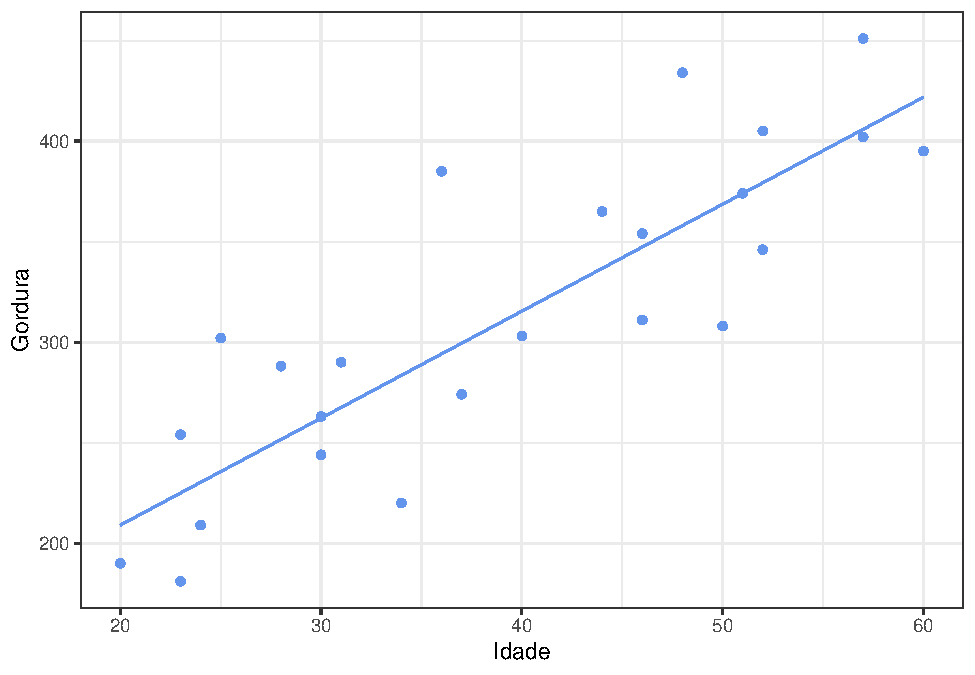
\includegraphics{novo_files/figure-latex/unnamed-chunk-4-1.pdf}

Sabemos que na matemática básica, a relação linear é descrita como:

\[Y_i = a+bX_i\] onde:\\
- \(Y\) são as \(i\) variáveis dependentes;\\
- \(a\) é o intercepto;\\
- \(b\) é o coeficiente angular; - \(X\) são as \(i\) variáveis
independetes;\\
- \(i=1,2,3...\).

No caso do exemplo, a relação entre Idade e Teor de Gordura no Sangue
pode ser descrita por:

\[\hat{y}_i = 102.6 + 5.3x_i\] ~

\hypertarget{modelo}{%
\section{1.1 Modelo}\label{modelo}}

Em regressão linear, a estrutura é quase a mesma. Mudamos o nome dos
parâmetros \(a\) e \(b\) para as letras gregas \(\beta_0\) e \(\beta_1\)
respectivamente e adicionamos o termo \(\varepsilon_i\), que vai
representar o erro (também chamado de ruído) de cada observação (já que,
quando coletamos determinado medida em um experimento, essa medição é
passivel de pequenos erros a cada coleta). Então, o \textbf{modelo de
regressão linear simples} é:onde:

\begin{itemize}
\tightlist
\item
  \(Y\) são as \(i\) variáveis independentes (ou resposta para a i-ésima
  obervação);\\
\item
  \(\beta_0\) é o intercepto;\\
\item
  \(\beta_1\) é o incremento de \(X_i\) em \(Y_i\);
\item
  \(X\) são as \(i\) variáveis independetes (ou conhecidas);
\item
  \(\varepsilon_i\) são os erros aleatórios associados a cada observação
  \(X_i\);
\item
  \(i=1,2,3...\).
\end{itemize}

\[Y_i =\beta_0+\beta_1X_i + \varepsilon_i\]

Quando aplicamos este modelo aos nosso dados, teremos os \textbf{valores
ajustados} ou \textbf{estimados}, i.e.:

\[\hat{Y_i}= \hat{\beta_0}+\hat{\beta_1}X_i\] Nestes valores ajustados
estão contidos os \textbf{resíduos}, que são a diferença entre o valor
verdadeiro da variável resposta e o valor estimado pelo modelo,
respectivamente:

\[\epsilon_i=Y_i-\hat{Y_i}\]
\[\qquad\qquad\quad=Y_i-\hat{\beta_0}+\hat{\beta_1}X_i\]

Vale lembrar que \textbf{erro} e \textbf{resíduo} não são a mesma coisa:

\begin{itemize}
\tightlist
\item
  O erro aleatório \(\varepsilon_i\) do modelo se refere ao contexto
  populacional, antes do ajuste do modelo e amostragem.
\item
  O resíduo \(\epsilon_i\) se refere ao contexto amostral, após o modelo
  ser ajustado com base na amostra coletada.
\end{itemize}

A primeira suposição a respeito deste modelo a respeito dos erros:

\begin{itemize}
\tightlist
\item
  O valor esperado dos erros é sempre zero:
  \(E[\varepsilon_i]=0 \quad\forall i\);\\
\item
  Sua variância é sempre constante
  \(Var[\varepsilon_i]=\sigma^2\quad\forall i\);\\
\item
  Eles não são correlacionados:
  \(Cov(\varepsilon_i, \varepsilon_j)=0 \quad \forall\quad i \ne j\).
\item
  Eles seguem a distribuição de probabilidade normal e são independentes
  e identicamente distribuidos:
  \(\varepsilon \stackrel{iid}{\sim} N(0, \sigma^2)\)
\end{itemize}

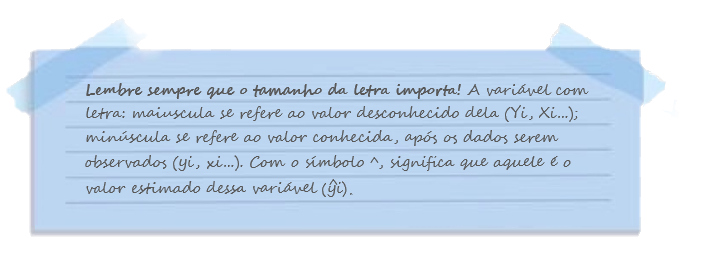
\includegraphics{images/note4.png}

Voltando ao exemplo, na figura abaixo temos as representações dos
parâmetros nas partes em destaque: \(\beta_0\) como intercepto, isto é,
ponto em que a reta corta o eixo \(Y\); \(\beta_1\) como incremento em
\(Y\) para cada uma unidade de \(X\); e por fim \(\varepsilon_i\) como a
distância entre a reta de regressão e a observação \(X_i\).

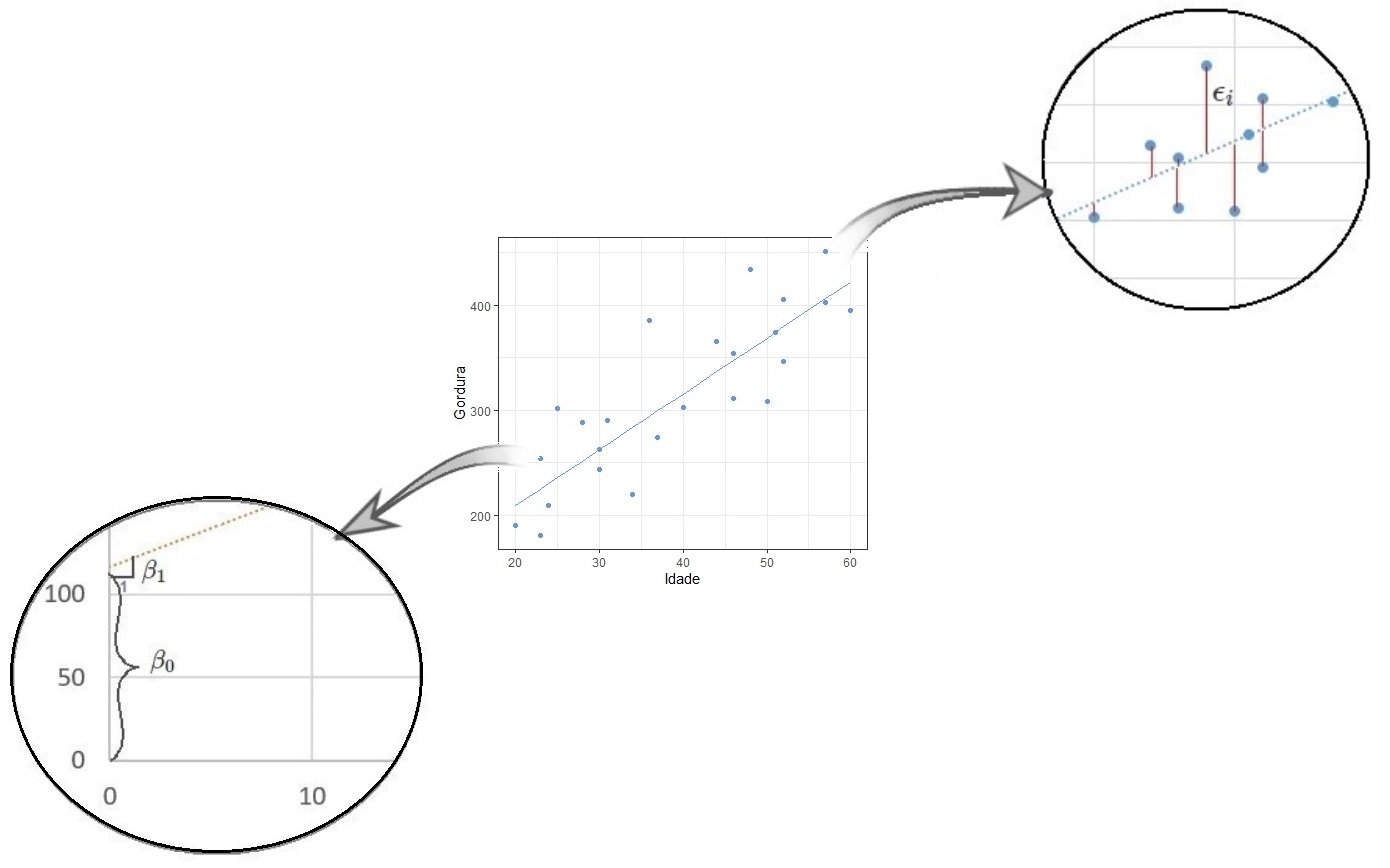
\includegraphics{images/denovo.jpeg}

Deste modo, nosso modelo de regressão linear simples que descreve a
relação entre idade e teor de gordura no sangue é:

\[\hat{y}_i = 102.6 + 5.3x_i+\varepsilon_i\] para \(i=1,2,...,24,25\).

~

\hypertarget{propriedades-do-modelo}{%
\section{1.2 Propriedades do modelo}\label{propriedades-do-modelo}}

Agora que conhecemos o modelo, vamos conferir algumas de suas
propriedades. Sabemos então qe \(Y_i\) são as variáveis resposta e que
\(\varepsilon_i\) são variáveis aleatórias correspondentes aos erros.
Como o valor esperado de \(\varepsilon_i\) é sempre zero, então:

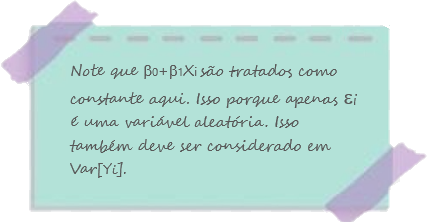
\includegraphics{images/note5.png}

\[E[Y_i]=E[\beta_0+\beta_1X_i+\varepsilon_i]\]
\[\qquad\quad=E[\beta_0+\beta_1X_i]+E[\varepsilon_i]\]
\[\qquad\quad=E[\beta_0+\beta_1X_i]+0\quad\]
\[\qquad=\beta_0+\beta_1X_i\quad\qquad\]

~

\(\qquad\qquad Var[Y_i]=Var[\beta_0+\beta_1X_i+\varepsilon_i]\)

\(\qquad\qquad\qquad\quad = Var[\varepsilon_i]\qquad\qquad\)

\(\qquad\qquad\qquad\quad = \sigma^2\qquad\qquad\)

Além disso, como os erros \(\varepsilon_i\) e \(\varepsilon_j\) não
correlacionados, então as respostas \(Y_i\) e \(Y_j\) também não serão.

\hypertarget{estimauxe7uxe3o-dos-paruxe2metros}{%
\section{1.2 Estimação dos
parâmetros}\label{estimauxe7uxe3o-dos-paruxe2metros}}

~

Mas afinal, como determinamos os valores de \(\beta_0\) e \(\beta_1\)?
Para resolver essa questão, temos dois métodos estatisticos: método de
mínimos quadrados e método da máxima verossimilhança. Em ambos o
objetivo é sempre encontrar um \(\beta_0\) e \(\beta_1\) que nos dê a
melhor reta em relação aos dados.

~

\hypertarget{muxe9todo-de-muxednimos-quadrados-mmq}{%
\section{1.2.1 Método de Mínimos Quadrados
(MMQ)}\label{muxe9todo-de-muxednimos-quadrados-mmq}}

~

Para encontrar a melhor reta, este método minimiza a soma dos erros
\(\varepsilon_i\), ou seja, a soma das distâncias entre a reta e os
dados coletados. Como estamos somando o tamanho desse erros, elevamos
seus valores ao quadrado, então temos:

\[\varepsilon_1^2+\varepsilon_2^2+\varepsilon_3^2+...+\varepsilon_n^2 = \sum_{i=1}^{n} \varepsilon_i^2\]

para \(i= 1,2,3,...n.\), i.e.~para n observações. Como
\(\varepsilon_i = Y_i-(\beta_0+\beta_1X_i)= Y_i-\beta_0-\beta_1X_i\),
então queremos encontrar um \(\beta_0\) e \(\beta_1\) tal que minimize
\(Q\):

\[Q=\sum_{i=1}^{n} \varepsilon_i^2=\sum_{i=1}^{n} (Y_i-\beta_0-\beta_1X_i)^2\]
Para encontrar essas estimativas analiticamente nos baseando no modelo
de regressão simples, usaremos as duas equações que seguem
abaixo,conjuntamente:

\[\sum_{i=1}^{n}Y_i = n\beta_0-\beta_1\sum_{i=1}^{n}X_i\]
\[\sum_{i=1}^{n}X_iY_i = \beta_0\sum_{i=1}^{n}X_i-\beta_1\sum_{i=1}^{n}X_i^2\]
Essa equações, também chamadas de equações normais, podem ser derivadas
em relação aos parâmetros:

\[\frac{\partial Q}{\partial \beta_0}=-2\sum_{i=1}^{n}(Y_i-\beta_0-\beta_1X_i)\]\\
\[\frac{\partial Q}{\partial \beta_1}=-2\sum_{i=1}^{n}X_i(Y_i-\beta_0-\beta_1X_i)\]

Igualando essas derivadas à zero, encontramos os valores de \(\beta_0\)
e \(\beta_1\) que minimizam \(Q\):

~


\includegraphics{images/note1.jpg}

\[-2\sum_{i=1}^{n}(Y_i-\hat{\beta}_0-\hat{\beta}_1X_i)=0\]
\[-2\sum_{i=1}^{n}X_i(Y_i-\hat{\beta}_0-\hat{\beta}_1X_i)=0\]

Dividindo os dois lados das equações por \(-2\):
\[\sum_{i=1}^{n}(Y_i-\hat{\beta}_0-\hat{\beta}_1X_i)=0\]
\[\sum_{i=1}^{n}X_i(Y_i-\hat{\beta}_0-\hat{\beta}_1X_i)=0\]

Expandindo as equações, conseguimos chegar nas equações normais:
\[\sum_{i=1}^{n}Y_i-n\hat{\beta}_0-\hat{\beta}_1\sum_{i=1}^{n}X_i=0\]
\[\sum_{i=1}^{n}X_iY_i-\hat{\beta}_0\sum_{i=1}^{n}X_i-\hat{\beta}_1\sum_{i=1}^{n}X_i^2=0\]

~

\(\qquad\qquad\qquad\qquad\qquad\qquad\qquad\qquad\qquad\)
\textbf{Equações Normais}

\[\sum_{i=1}^{n}Y_i\quad=n\hat{\beta}_0+\hat{\beta}_1\sum_{i=1}^{n}X_i\]
\[\sum_{i=1}^{n}X_iY_i\quad=\hat{\beta}_0\sum_{i=1}^{n}X_i+\hat{\beta}_1\sum_{i=1}^{n}X_i^2\]

~

A partir delas conseguim ao isolar os parâmetros e obter as estimações.
Para mais detalhes desta etapa, veja a
\href{https://larissars.github.io/Apostilas-estatistica/apendice.html\#Demonstração_1}{Apêndice:
Demonstração 1}.

~

\[\hat{\beta}_0=\bar{Y}-\beta_1\bar{X}\]

\[\hat{\beta}_1 = \frac{\sum_{i=1}^{n}(X_i-\bar{X})(Y_i-\bar{Y})}{\sum_{i=1}^{n}(X_i-\bar{X})}\]

As \textbf{vantagens} do método dos mínimos quadrados é que, além de ser
comumente usado, ele é comportado pelos programas de estatística de modo
geral.\\
Entretanto, precisamos de certos \textbf{requisitos} para poder usar
ele:

\begin{itemize}
\tightlist
\item
  \textbf{Lineariedade dos dados:} seu comportamento pode ser decrito
  por uma reta
\end{itemize}

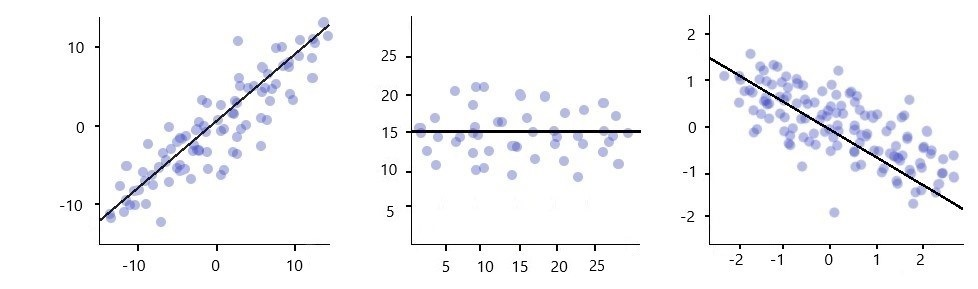
\includegraphics{images/regressoes.jpg}

\begin{itemize}
\tightlist
\item
  \textbf{Normalidade dos resíduos:} os resíduos do modelo seguem uma
  distribuição aproximadamente normal, i.e.,
  \(\epsilon \cong N(\mu, \sigma^2)\).
\end{itemize}

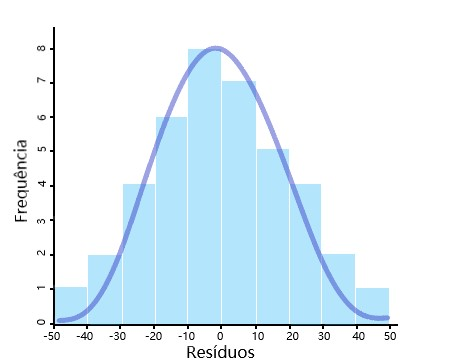
\includegraphics{images/resinorm.jpg}

\begin{itemize}
\tightlist
\item
  \textbf{Homocedasticidade:} a variabilidade dos resíduos é constante.,
  ou seja, \(Var(\epsilon)=c\).
\end{itemize}

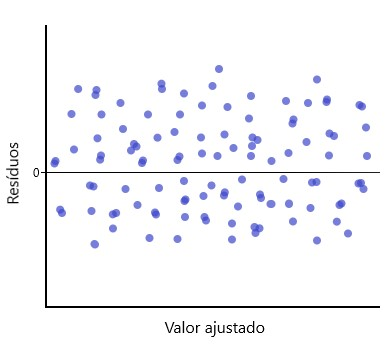
\includegraphics{images/homoresi.jpg}

\begin{itemize}
\tightlist
\item
  \textbf{Erros sem autocorrelação:} Os valores ordenados não tem
  relação com o espaço ou tempo. Matematicamente, \(\epsilon_i\) e
  \(\epsilon_j\) tem \(Cov(\epsilon_i, \epsilon_j)=0, \forall i \ne j\).
\end{itemize}

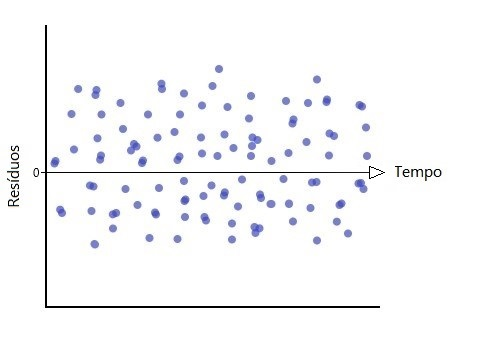
\includegraphics{images/autocor.jpg}

\hypertarget{propriedades-dos-estimadores-de-mmq}{%
\section{1.2.1.1 Propriedades dos estimadores de
MMQ}\label{propriedades-dos-estimadores-de-mmq}}

Os estimadores \(\hat{\beta}\) obtidos pelo método de método de mínimos
quadrados são funções lineares de Y
(\href{https://larissars.github.io/Apostilas-estatistica/apendice.html\#Demonstração_2}{Apêndice:
Demonstação 2}). E segundo o Teorema de Gauss Markov, dado as condições
do modelo de regressão linear, o método de mínimos quadrados:

\begin{itemize}
\item
  Tem estimadores \(\beta_0\) e \(\beta_1\) não viesados, i.e., o valor
  esperado do estimador é ao próprio arametro que foi estimado:
  \(E[\hat{\beta_0}]= \beta_0\) e \(E[\hat{\beta_1}]= \beta_1\). Isso
  acontece independente da distribuição de probabilidade desses erros
  (\href{https://larissars.github.io/Apostilas-estatistica/apendice.html\#Demonstração_3}{Apêndice:
  Demonstação 3}).
\item
  Tem variância mínima entre todos os estimadores não viesados e
  lineares.
\end{itemize}

\[Var[\hat{\beta_0}]=\sigma^2\Bigg[\frac{1}{n}+\frac{\bar{X}^2}{\sum_{i=0}^{n}(X_i-\bar{X}^2)}\Bigg]\]

\[Var[\hat{\beta_1}]=\frac{\sigma^2}{\sum_{i=0}^{n}(X_i-\bar{X})^2}\]

Logo eles são os mais precisos entre esse tipo de estimador.

\begin{itemize}
\tightlist
\item
  Os estimadores de mínimos quadrados tem distribuição de probabilidade
  Normal.
\end{itemize}

\[\hat{\beta_0} \sim N\Bigg(\beta_0, \sigma^2\Bigg[\frac{1}{n}+\frac{\bar{X}^2}{\sum_{i=0}^{n}(X_i-\bar{X}^2)}\Bigg]\Bigg)\]

\[\hat{\beta_0} \sim N\Bigg(\beta_1,\frac{\sigma^2}{\sum_{i=0}^{n}(X_i-\bar{X}^2)} \Bigg)\]

Além disso, temos que:

\begin{itemize}
\tightlist
\item
  Considerando \(\sum_{i=1}^{n}(X_i-\bar{X})(Y_i-\bar{Y})=S_{xy}\) como
  a soma dos produtos de X e Y, \(\sum_{i=1}^{n}(X_i-\bar{X})=S_{XX}\)
  como a soma dos quadrados de X, podemos afirmar que:
\end{itemize}

\[\hat{\beta}_1 = \frac{\sum_{i=1}^{n}(X_i-\bar{X})(Y_i-\bar{Y})}{\sum_{i=1}^{n}(X_i-\bar{X})}=\frac{S_{xy}}{S_{xx}}\]

\begin{itemize}
\item
  Esses estimadores são funções lineares das observações das variáveis
  resposta \(y_i\).
\item
  Suas variâncias são proporcionais as variâncias dos erros
\item
  São estimadores correlacionados
\end{itemize}

Veja mais detalhes sobre os resultados acima em \href{}{Demonstração X}.

\hypertarget{exemplo-no-r}{%
\section{1.2.1.3 Exemplo no R}\label{exemplo-no-r}}

Para reproduzir o exemplo exibido no inicio do capítulo, precisaremos
carregar os pacotes \emph{readr} e \emph{ggplot2}.

\begin{Shaded}
\begin{Highlighting}[]
\CommentTok{\#carregando os pacotes necessários}
\FunctionTok{library}\NormalTok{(}\StringTok{"readr"}\NormalTok{)}
\FunctionTok{library}\NormalTok{(}\StringTok{"ggplot2"}\NormalTok{)}
\end{Highlighting}
\end{Shaded}

Em seguidas vamos ler os dados obtidos na
\href{https://people.sc.fsu.edu/~jburkardt/datasets/regression/x09.txt}{página}.

\begin{Shaded}
\begin{Highlighting}[]
\NormalTok{dados }\OtherTok{=} \FunctionTok{read\_table2}\NormalTok{(}\StringTok{"https://people.sc.fsu.edu/\textasciitilde{}jburkardt/datasets/regression/x09.txt"}\NormalTok{, }\AttributeTok{col\_names =} \ConstantTok{FALSE}\NormalTok{ ,}\AttributeTok{skip =} \DecValTok{36}\NormalTok{) }\CommentTok{\#lendo apenas a tabela de dados }

\NormalTok{dados }\OtherTok{=}\NormalTok{ dados[,}\FunctionTok{c}\NormalTok{(}\DecValTok{4}\NormalTok{,}\DecValTok{5}\NormalTok{)]}\CommentTok{\#seleciona as duas ultimas colunas}

\FunctionTok{colnames}\NormalTok{(dados) }\OtherTok{=} \FunctionTok{c}\NormalTok{(}\StringTok{"Idade"}\NormalTok{, }\StringTok{"Gordura"}\NormalTok{) }\CommentTok{\#renomendo as colunas}

\FunctionTok{head}\NormalTok{(dados) }\CommentTok{\#Mostra as 6 primeiras linhas da tabela}
\end{Highlighting}
\end{Shaded}

\begin{verbatim}
## # A tibble: 6 x 2
##   Idade Gordura
##   <dbl>   <dbl>
## 1    46     354
## 2    20     190
## 3    52     405
## 4    30     263
## 5    57     451
## 6    25     302
\end{verbatim}

Com os dados já separados, ajustaremos um modelo de regressão linear
simples.

\begin{Shaded}
\begin{Highlighting}[]
\NormalTok{ajuste }\OtherTok{\textless{}{-}} \FunctionTok{lm}\NormalTok{(Gordura }\SpecialCharTok{\textasciitilde{}}\NormalTok{ Idade, dados) }\CommentTok{\#ajuste do modelo}
\FunctionTok{summary}\NormalTok{(ajuste) }\CommentTok{\#exibe os resultados detalhados do ajuste}
\end{Highlighting}
\end{Shaded}

\begin{verbatim}
## 
## Call:
## lm(formula = Gordura ~ Idade, data = dados)
## 
## Residuals:
##     Min      1Q  Median      3Q     Max 
## -63.478 -26.816  -3.854  28.315  90.881 
## 
## Coefficients:
##             Estimate Std. Error t value Pr(>|t|)    
## (Intercept) 102.5751    29.6376   3.461  0.00212 ** 
## Idade         5.3207     0.7243   7.346 1.79e-07 ***
## ---
## Signif. codes:  0 '***' 0.001 '**' 0.01 '*' 0.05 '.' 0.1 ' ' 1
## 
## Residual standard error: 43.46 on 23 degrees of freedom
## Multiple R-squared:  0.7012, Adjusted R-squared:  0.6882 
## F-statistic: 53.96 on 1 and 23 DF,  p-value: 1.794e-07
\end{verbatim}

Dado dos coeficientes do ajuste, ambos significativos, temos o modelo

\[\hat{y}_i = 102.6 + 5.3x_i\]

E partir dele, podemos fazer o gráfico da reta dos valores preditos
sobre os valores observados.

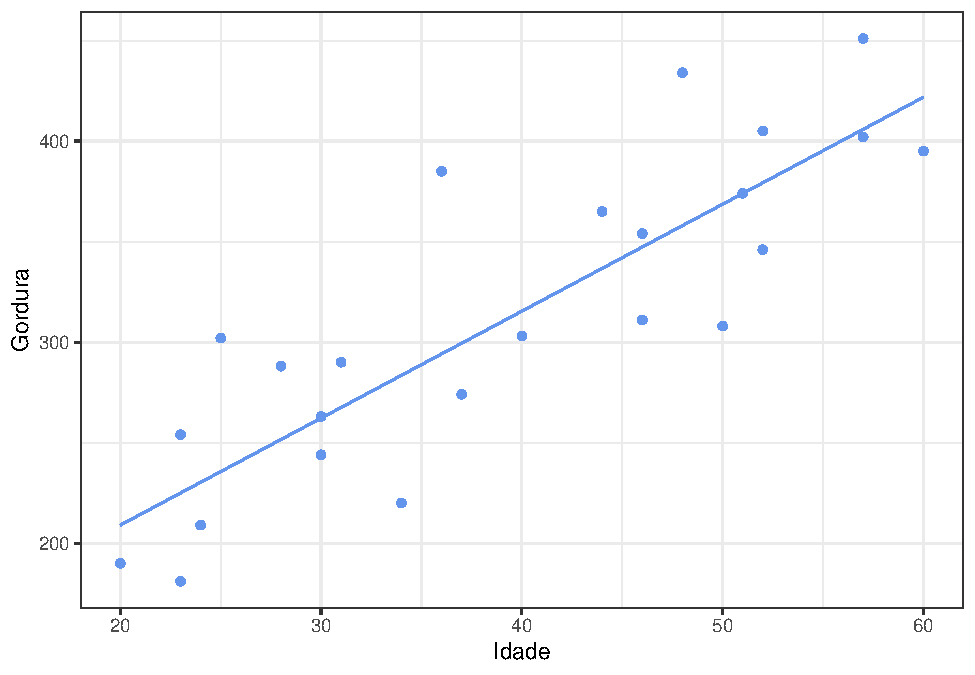
\includegraphics{novo_files/figure-latex/unnamed-chunk-8-1.pdf}

~

\hypertarget{muxe9todo-da-muxe1xima-verossimilhanuxe7a-mmv}{%
\section{1.2.2 Método da Máxima Verossimilhança
(MMV)}\label{muxe9todo-da-muxe1xima-verossimilhanuxe7a-mmv}}

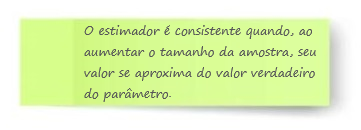
\includegraphics{images/note7.png}

O método de máxima verossilimilhança utiliza o produtos das densidades
das distribuição de probabilidade de \(Y_i\) como uma medida para a
consistência dos parâmetros para aquela amostra. Assim o método escolhe
os valores máximos da verossimilhança estimada, tal que os valores dos
paramêtros sejam mais consistentes.

Aqui, por ser mais simples, usaremos a log-verossimilhança negartiva.
Partindo do fato que \(E(Y_i) = \beta_0-\beta_1X_i\) e
\(Var[Y_i]=\sigma^2\), então a função densidade de probabilidade de
\(Y_i\) será:

\[f_i=\frac{1}{\sqrt {2\pi\sigma} }exp\bigg[-\frac{1}{2}\bigg(\frac{Y_i-\beta_0-\beta_1X_i}{\sigma}\bigg)^2 \bigg]\]

Fazendo o produtório das n densidades, correspondentes a cada uma das n
observações, temos a função de máxima verossimilhança. Nela consideramos
que a variância dos erros de cada observação é desconhecida:

\[\mathcal{L}(\beta_o, \beta_1, \sigma^2)=  \prod_{i=1}^{n} \frac{1}{(2\pi\sigma^2)^{1/2}}exp\bigg[-\frac{1}{2\sigma^2}(Y_i-\beta_0-\beta_1X_i)^2 \bigg]\]
Simplificando a equação temos:
\[\mathcal{L}(\beta_o, \beta_1, \sigma^2)=\frac{1}{(2\pi\sigma^2)^{n/2}}exp\bigg[ -\frac{1}{2\sigma^2}\sum_{i=1}^{n}(Y_i-\beta_0-\beta_1X_i)^2\bigg]\]

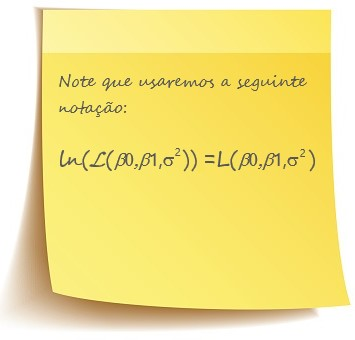
\includegraphics{images/note2.jpg}

Para encontrar as estimativas dos parâmetros precisaremos fazer as
derivadas parciais de \(L(\beta_o, \beta_1, \sigma^2)\) em relação a
cada parâmetro. Como \(L(\beta_o, \beta_1, \sigma^2)\) e
\(ln(\mathcal{L}(\beta_o, \beta_1, \sigma^2))\) são equações que
maximizam a verossimilhança, podemos trabalhar com ambos. Note que
usaremos a seguinte notação:

\[L(\beta_o, \beta_1, \sigma^2) = -\frac{n}{2} ln( 2\pi) -\frac{n}{2} ln(\sigma^2)-\frac{1}{2\sigma^2}\sum_{i=1}^{n}(y_i-\beta_0-\beta_1x_i)^2\]

Mas escolhemos o logaritmo da função de máxima verossimilhança por ser
mais facil de derivar. Seguem as derivadas particias dos parâmetros, já
igualadas a zero:

~

\[\frac{\partial L(\beta_o, \beta_1, \sigma^2)}{\partial \beta_0}\quad= -\frac{1}{\sigma^2}\sum_{i=1}^{n}(y_i-\beta_0-\beta_1x_i)=0\]

\[\quad\quad=\sum_{i=1}^{n}(y_i-\beta_0-\beta_1x_i)=0\]
\[\sum_{i=1}^{n}y_i=n\beta_0+(\sum_{i=1}^{n}x_i)\beta_1\]
\[\hat{\beta}_0=\bar{Y}-\beta_1\bar{X}\]

~

\[\frac{\partial L(\beta_o, \beta_1, \sigma^2)}{\partial \beta_1} \quad= -\frac{1}{\sigma^2}\sum_{i=1}^{n}(y_i-\beta_0-\beta_1x_i)=0\]
\[\quad\quad\quad\quad\quad\quad=\sum_{i=1}^{n}(y_i-\beta_0-\beta_1x_i)x_i=0\]
\[\sum_{i=1}^{n}y_ix_i=(\sum_{i=1}^{n}x_i)\beta_0+(\sum_{i=1}^{n}x_i^2)\beta_1  \]

\[\hat{\beta}_1 = \frac{\sum_{i=1}^{n}(X_i-\bar{X})(Y_i-\bar{Y})}{\sum_{i=1}^{n}(X_i-\bar{X})}\]

~

\[\frac{\partial L(\beta_o, \beta_1, \sigma^2)}{\partial \sigma^2}=\frac{n}{\hat{\sigma}^2}-\frac{1}{\hat{\sigma}^4}\sum_{i=1}^{n}(Y_i-\beta_0-\beta_1X_i)=0\]

\[\frac{n}{\hat{\sigma}^2}=\frac{1}{\hat{\sigma}^4}\sum_{i=1}^{n}(Y_i-\beta_0-\beta_1X_i)\]
\[n=\frac{1}{\hat{\sigma}^2}\sum_{i=1}^{n}(Y_i-\beta_0-\beta_1X_i)\]

\[\hat{\sigma}^2=\frac{1}{n}\sum_{i=1}^{n}(Y_i-\beta_0-\beta_1X_i)^2\]
Como \(\hat{Y}_i=\beta_0-\beta_1X_i\), então:

\[\hat{\sigma}^2=\frac{\sum_{i=1}^{n}(Y_i-\hat{Y}_i)^2}{n}\]

\hypertarget{propriedades-dos-estimadores-de-mmv}{%
\section{1.2.2.1 Propriedades dos estimadores de
(MMV)}\label{propriedades-dos-estimadores-de-mmv}}

Esse estimador é do tipo um estimador viesado para p parâmetro da
variância \(E[\hat{\sigma^2}]=\frac{n-1}{n}\sigma^2\). Mas medida que n
cresce, \(\hat{\sigma^2}\) tende a ser não viesado:

\[lim_{n \to \infty }E[\hat{\sigma^2}]=lim_{n \to \infty} \frac{n-1}{n}\sigma^2=\sigma^2\]

Contudo ele é muito confiavel devido algumas propriedades:

\begin{itemize}
\tightlist
\item
  Consistência;
\item
  Eficiência Assintótica;
\item
  Normalidade Assimptótica;
\item
  Invariância.
\end{itemize}

\hypertarget{anuxe1lise-de-resuxedduos}{%
\section{1.3 Análise de Resíduos}\label{anuxe1lise-de-resuxedduos}}

Como já citado anteriormente, os resíduos são a diferença entre o valor
verdadeiro da variável resposta e o valor estimado pelo modelo,
respectivamente:

\[\epsilon_i=Y_i-\hat{Y_i}\] Eles são usados para avaliar o quão bom é o
ajuste do modelo, já que, toda variabilidade não explicada pelo modelo,
vai para os resíduos. Para isso vamos verificar seis caracteristicas:

\begin{itemize}
\tightlist
\item
  Se a regressão ajustada é uma função linear;
\item
  Se os erros tem variância constante;
\item
  Se os erros são independentes;
\item
  Se os erros tem distribuição normal;
\item
  Se o modelo não se ajusta para alguns outliers;
\item
  Se uma ou mais variaveis preditoras podem ser retiradas do modelo.
\end{itemize}

Um dos gráficos mais usados para avaliar se a função é linear e foi bem
ajustada é o gráfico de pontos dos resíduos pelos valores ajustados:

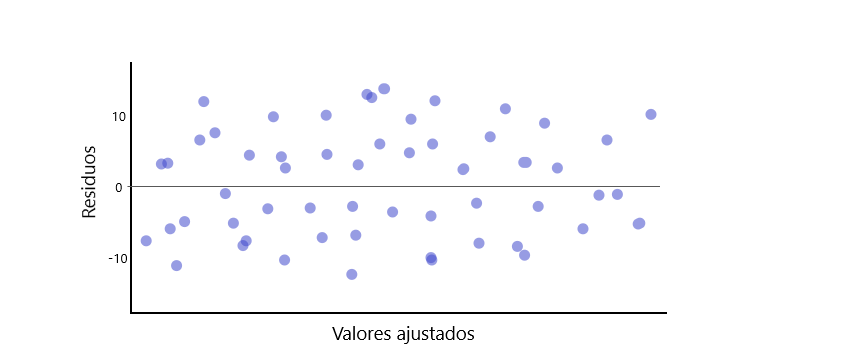
\includegraphics{images/residuos1.png}

Em um ajuste satisfatório teremos pontos aleatórios em torno da reta
horizontal (que marca o resíduo igual a zero) e que variam de forma
constante, como na figura (a). Quando isso não acontece (como nas demais
imagens), temos resíduos viesados, os quais podem nos dar pistas sobre o
comportamento não captado pelo modelo ajustado. Por exemplo, na figura
(b) temos uma comportamento claramento quadrático e na figura (c) uma
tendência linear positiva, essas caracteristicas não devem aparecer nos
resíduos e sim no modelo ajustado. Se você se deparar com essa situação,
refaça seu modelo.

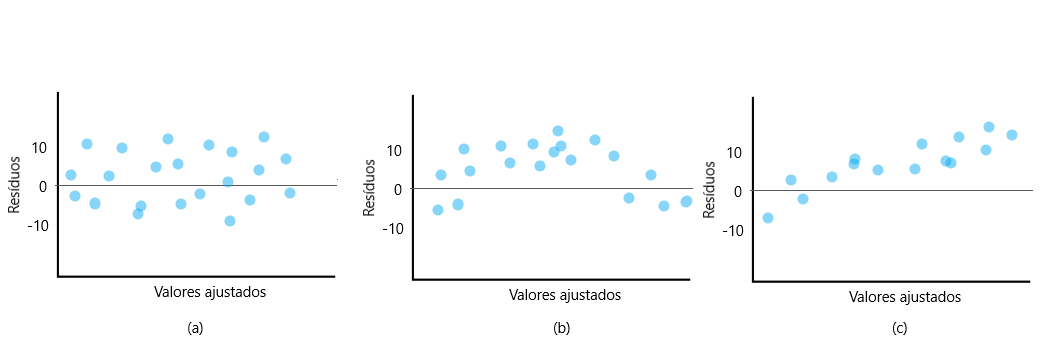
\includegraphics{images/residuos2.png}

Além disso é importante lembrar que, quando o valor de um i-ésimo
resíduo \(\epsilon_i\) for:

\begin{itemize}
\tightlist
\item
  Positivo, significa que o modelo subestimou a observação
\end{itemize}

\[\epsilon_i>0 \quad \to \quad Y_i-\hat{Y_i}>0 \quad \to \quad Y_i>\hat{Y_i}\]

\begin{itemize}
\tightlist
\item
  Negativo, significa que o modelo superestimou a observação
\end{itemize}

\[\epsilon_i<0 \quad \to \quad Y_i-\hat{Y_i}<0 \quad \to \quad Y_i<\hat{Y_i}\]
Outro gráfico importante é o dos resíduos absolutos (ou residuos ao
quadrado) versus a variável X (preditora) ou os valores ajustados de Y
(i.e.~\(\hat Y\)). Este gráfico é util para checarmos a variância dos
resíduos é ou não constante, bem como a presença de outliers.

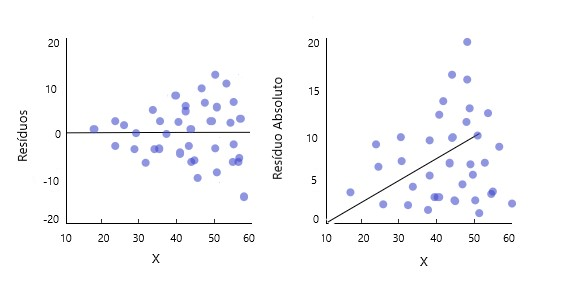
\includegraphics{images/residuos4.JPG}

Já a independência dos erros pode ser avaliada pelo simples gráfico de
pontos dos resíduos em relação a variável preditora ou em relação ao
tempo, pois com eles conseguimos ver se há a relação de um i-ésimo
resíduo com os demais próximos a ele.

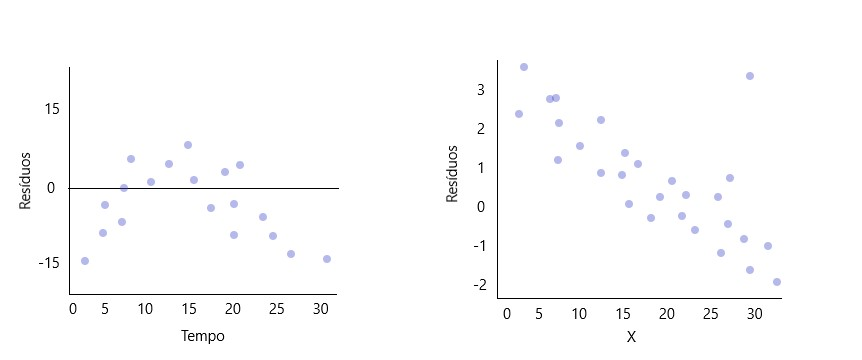
\includegraphics{images/residuos5.JPG}

Por fim e não menos importante, devemos checar a normalidade dos
resíduos. Isso pode ser feito por diversos gráficos: gráfico da
distribuição (Box plot, histograma, gráfico de pontos ou gráfico de
ramos e folhas); gráfico de comparação de frequências; gráfico de
normalidade dos resíduos (o mais usado).

\hypertarget{correlauxe7uxe3o}{%
\section{1.3.1 Correlação}\label{correlauxe7uxe3o}}

As relações entre as variáveis ajustadas no modelo podem ser fortes ou
fracas e avaliar essa força é muito importante para a avaliação do
modelo. Uma forma de quantificar essa força é pelo \textbf{correlação},
denotada pela letra R. Suponha que temos um conjunto de dados
\((x_1,y_1),(x_2,y_2),...,(x_n,y_n)\), sua correlação é dada por:

\[R = \frac{1}{n-1}\sum_{i=1}^{n} \frac{x_i-\bar{x}}{s_x} \frac{y_i-\bar{y}}{s_y}\]
onde \(\bar{x}\), \(\bar{y}\), \({s_x}\) e \({s_y}\) são respectivamente
as médias e desvio padrão amostral das variáveis x e y.

Os valores de R serão sempre entre -1 e 1. Quanto mais próximo de 1,
mais forte é a correlação linear positiva entre as variáveis. E quanto
mais próximo de -1, maior é a correlação linear negativa entre as
mesmas. Abaixo temos a imagem que representa as duas situações: em (a)
temos três casos de correlação linear positiva e em (b) temos os casos
para correlação linear negativa.

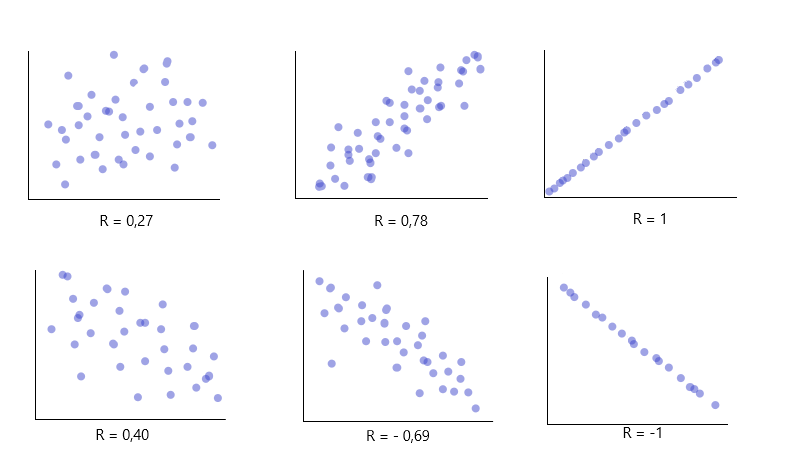
\includegraphics{images/residuos3.png}

\hypertarget{coeficiente-de-determinauxe7uxe3o}{%
\section{1.3.1 Coeficiente de
Determinação}\label{coeficiente-de-determinauxe7uxe3o}}

R² ajustado

\hypertarget{anuxe1lise-de-variuxe2ncia}{%
\section{Análise de Variância}\label{anuxe1lise-de-variuxe2ncia}}

Applied regresion pag 52,65-68 Applied Linear Statistical Models 5th pag
87-97

a)pq fazer b)exemplos c)como fazer

Applied Linear Statistical Models 5th pag 98

Applied regresion pag 55/64-65

\hypertarget{intervalos-de-confianuxe7a}{%
\subsubsection{Intervalos de
confiança}\label{intervalos-de-confianuxe7a}}

Applied Linear Statistical Models 5th pag 68,73-78

Applied regression pag 58,59

\begin{verbatim}
  a)  exemplos de uso
  b) como fazer
\end{verbatim}

\hypertarget{teste-de-hipuxf3tese}{%
\subsubsection{Teste de Hipótese}\label{teste-de-hipuxf3tese}}

\begin{verbatim}
  a)  exemplos de uso
  b) como fazer
\end{verbatim}

\hypertarget{prediuxe7uxe3o}{%
\subsubsection{Predição}\label{prediuxe7uxe3o}}

\begin{verbatim}
  a)  exemplos de uso
  b) como fazer
\end{verbatim}

\hypertarget{diagnostico}{%
\subsubsection{Diagnostico}\label{diagnostico}}

a)pq fazer b)como fazer \#\#\# Transformações a)pq fazer b)exemplos
c)como fazer

~

\begin{center}\rule{0.5\linewidth}{0.5pt}\end{center}

+999999999 \#\# Regressão Linear Multipla

\hypertarget{forma-matricial}{%
\subsubsection{Forma matricial}\label{forma-matricial}}

\hypertarget{estimauxe7uxe3o-dos-paruxe2metros-1}{%
\subsubsection{Estimação dos
parâmetros}\label{estimauxe7uxe3o-dos-paruxe2metros-1}}

\hypertarget{anuxe1lise-de-variuxe2ncia-1}{%
\subsubsection{Análise de
Variância}\label{anuxe1lise-de-variuxe2ncia-1}}

\hypertarget{prediuxe7uxe3o-1}{%
\subsubsection{Predição}\label{prediuxe7uxe3o-1}}

\hypertarget{teste-de-hipuxf3tese-1}{%
\subsubsection{Teste de Hipótese}\label{teste-de-hipuxf3tese-1}}

\hypertarget{intervalo-de-confianuxe7a}{%
\subsubsection{Intervalo de Confiança}\label{intervalo-de-confianuxe7a}}

Soma extra de quadrados(?)\\
Coef de determinação parcial (?)\\
Reg multi padronizada (?)\\
Multicolineariedade(?)\\
Medidas de influência e Alavancagem (?) *Caio

~

\hypertarget{regressuxe3o-polinomial}{%
\subsection{Regressão Polinomial}\label{regressuxe3o-polinomial}}

Regressão com intervenção (?)\\
Região de confiança (?)\\
Teste de Hip Linear (?)

~

\hypertarget{seleuxe7uxe3o-de-modelos}{%
\subsection{Seleção de modelos}\label{seleuxe7uxe3o-de-modelos}}

Regressão Parcial (?)\\
Inflação da variância (?)

~

\hypertarget{regressuxe3o-nuxe3o-linear}{%
\subsection{Regressão Não-Linear}\label{regressuxe3o-nuxe3o-linear}}

Regressão logistica(?) *openintro

\hypertarget{referuxeancia}{%
\section{Referência}\label{referuxeancia}}

~

\begin{itemize}
\tightlist
\item
  Análise de Regressão
\end{itemize}

\textbf{Azevedo, Caio L. N.}. ME 613A - Análise de regressão, Primeiro
Semestre 2019. IMECC - UNICAMP. Disponível em:
\url{https://www.ime.unicamp.br/~cnaber/Material_ME613_1S_2019.htm}.
Acessado em: Julho à X de 2021

\textbf{Carvalho, B}. ME613: Análise de Regressão. Github. 2021.
Disponível em: \url{http://me613-unicamp.github.io/}. Acessado em: Julho
à X de 2021

\textbf{Caffo, B}. (2019). Regression models for data science in R.
Leanpub. 2019. Disponível em: \url{https://leanpub.com/regmods/read}.
Acessado em: Julho à X de 2021

\textbf{Diez, D.; Rundel, M. C.; Barr, C. D.}. Openintro Statistics.
Quarta edição. Atualizado em 12 de Novembro de 2019. Versão online
gratuita. Disponível em: \url{https://www.openintro.org/book/os/}.
Acessado em: Julho à X de 2021

\textbf{Kutner, M. H.; Nachtsheim, C. J.;Neter, J.; Li, W.}.Applied
Linear Statistical Models. Quinta edição. 2005.

João L. F. Batista. Análise de Regressão Aplicada.2004. Departamento de
Ciências Florestais ESALQ - USP

\url{http://www.leg.ufpr.br/~paulojus/embrapa/Rembrapa/Rembrapase19.html}

\end{document}
